\documentclass[11pt, twoside]{report}

\usepackage{fontspec}
\usepackage[utf8]{inputenc}
\usepackage[bitstream-charter]{mathdesign}
\usepackage{bbding}
\usepackage{ragged2e}
\usepackage{parskip}
\usepackage{enumitem}
\usepackage{titlesec}
\usepackage{paracol}
\usepackage{mdframed}
\usepackage[margin=1in]{geometry}

\usepackage[autocompile]{gregoriotex}

\titleformat{\chapter}[block]{\huge\scshape\filcenter}{}{1em}{}
\titleformat{\section}[block]{\Large\bfseries\filcenter}{}{1em}{}

\mdfsetup{skipabove=\topskip, skipbelow=\topskip}

\newcommand{\rubric}[1]{
	\switchcolumn[0] {
		\itshape
		#1
	}
}

\newcommand{\latinenglish}[2]{
	\switchcolumn[0]* {
		#1
	}
	\switchcolumn[1] {
		\itshape\small
		#2
	}
}

\newcommand{\latinenglishequal}[2]{
	\switchcolumn[0]* {
		#1
	}
	\switchcolumn[1] {
		\itshape
		#2
	}
}

\newenvironment{latinenglishsection}
	{\columnratio{.65, .35} \begin{paracol}{2}}
	{\end{paracol}}

\newenvironment{latinenglishequalsection}
	{\columnratio{.5, .5}\begin{paracol}{2}}
	{\end{paracol}}

\setlength{\columnseprule}{0.4pt}

\newcommand{\heading}[1]{
	\begin{leftcolumn}
		#1
	\end{leftcolumn}
}

\newcommand{\spanning}[1]{
	\switchcolumn*[#1]
}

\newenvironment{verses}[1]
	{\begin{flushleft} \begin{enumerate}[leftmargin=*] \setcounter{enumi}{#1}}
	{\end{enumerate} \end{flushleft}}

\newenvironment{versicles}{\par\leavevmode\parskip=0pt}{}

\newenvironment{collect}
{
	\leavevmode
	\parindent=1em
	\parskip=0pt
	\noindent Orémus.\par
}{}

\newenvironment{optionbox}
{
	\switchcolumn[0]
	\begin{mdframed}
%	\begin{minipage}{0.8\linewidth}
}{
%	\end{minipage}
	\end{mdframed}
}

\newcommand{\optionrule}{
	\begin{center}
	\rule{0.5\linewidth}{0.6pt}
	\end{center}
}

\newenvironment{optionruled}
{
	\optionrule
}
{
	\optionrule
}

% for use inside the collect environment
\newcommand{\Amen}{\par\noindent \Rbar. Amen.}

\begin{document}

\vspace*{4cm}

\begin{center}
	\textbf{\Huge Traditional Exorcism and Blessing of St. Benedict's Medal}\\
	%{\LARGE According to the Washtenaw Use}
\end{center}

\vspace{0.5cm}
% REFERENCE: http://www.traditionalcatholicpriest.com/2014/03/21/traditional-catholic-latin-exorcism-and-blessing-of-saint-benedicts-medal/

\begin{center}
	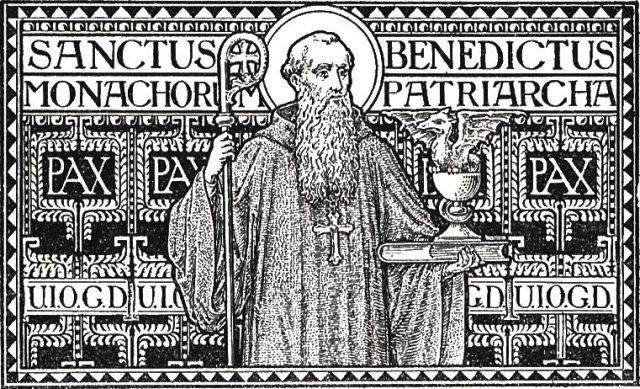
\includegraphics[width=\textwidth]{StBenedict.jpg}
\end{center}

\vfill\pagebreak

%\vspace*{7.5cm}
%Herein follows the traditional formula for exorcising and blessing the medal of St. Benedict. The formula can be found in the Roman Ritual.

%\vfill\pagebreak
 
\section*{Exorcism}

Prior to the administering of the exorcism and blessing, Holy Water must be obtained and nearby for use.

\begin{latinenglishsection}

\latinenglish{
	{\color{red}\Rbar.} Adjutorium nostrum in nomine Domini.
	
	{\color{red}\Vbar.} Qui fecit caelum et terram.
	
	{\color{red} The priest exorcises the medals, making the Sign of the Cross four times: once after `Deum' and thrice when invoking the Holy Trinity.}
	
	Exorcizo vos, numismata, per Deum {\color{red}\maltese} Patrem omnipotentem, qui fecit caelum et terram, mare et omnia, quae in eis sunt.  Omnis virtus adversarii, omnis exercitus diaboli, et omnis incursus, omne phantasma satanae, eradicare et effugare, ab his numismatibus: ut fiant omnibus, qui eis usuri sunt, salus mentis et corporis: in nomine Patris {\color{red}\maltese} omnipotentis, et Jesu {\color{red}\maltese} Christi Filii ejus, Domini nostri, et Spiritus {\color{red}\maltese} Sancti Paracliti, et in caritate ejusdem Domini nostri Jesu Christi, qui venturus est judicare vivos et mortuos, et saeculum per ignem. 
	
	{\color{red}\Rbar.} Amen.
}{
	{\color{red}\Rbar.} Our help is in the Name of The Lord.
	
	{\color{red}\Vbar.} Who made Heaven and earth.
	
	 In the name of God the Father {\color{red}\maltese} who made heaven and earth, the seas and all that is in them, I exorcise this medal against the power and attacks of the evil one.  May all who use this medal devoutly be blessed with health of soul and body.  In the name of the Father {\color{red}\maltese} almighty, of the Son {\color{red}\maltese} Jesus Christ our lord, and of the Holy {\color{red}\GreDagger}  Spirit the Paraclete, and in the love of the same Lord Jesus Christ who will come on the last day to judge the living and the dead, and the world by fire.
	 
	{\color{red}\Rbar.} Amen.
}

\end{latinenglishsection}

\section*{Blessing}

\begin{latinenglishsection}

\latinenglish{
	{\color{red}\Vbar.} Domine exaudi orationem meam.
	
	{\color{red}\Rbar.} Et clamor meus ad te veniat.
	
	{\color{red}\Vbar.} Dominus vobiscum.
	
	{\color{red}\Rbar.} Et cum spiritu tuo.
	
	Oremus:  Deus omnipotens, bonorum omnium largitor, supplices te rogamus, ut per intercessionem sancti Benedicti his sacris numismatibus tuam beneditionem {\color{red}\maltese} infundas, ut omnes qui ea gestaverint ac bonis operibus intenti fuerint, sanitatem mentis et corporis, et gratiam sanctificationis, atque indulgentias (nobis) concessas consequi mereantur, omnesque diaboli insidias et fraudes, per auxilium misericordiae tuae, studeant devitare et in conspectu tuo sancti et immaculati valeant apparere.  Per Christum Dominum nostrum.  
	
	{\color{red}\Rbar.} Amen.
}{
	{\color{red}\Vbar.} O Lord hear my prayer.
	
	{\color{red}\Rbar.} And let my cry come unto Thee.
	
	{\color{red}\Vbar.} The Lord be with you.
	
	{\color{red}\Rbar.} And with Thy spirit.
	
	Let us pray:  Almighty God, the boundless source of all good things, we humbly ask that, through the intercession of St. Benedict, you pour out your blessings {\color{red}\maltese} upon this medal.  May those who use it devoutly and earnestly strive to perform good works, be blessed by you with health of soul and body, the grace of a holy life, and remission of the temporal punishment due to sin.  May they also with the help of your merciful love, resist the temptation of the evil one and strive to exercise true charity and justice toward all, so that one day they may appear sinless and holy in you sight. This we ask through Christ our Lord. 
	
	{\color{red}\Rbar.} Amen.
}

\rubric{\color{red}The priest sprinkles the medal(s) with Holy Water.}

\end{latinenglishsection}

\end{document}